\chapter{Preliminars}
\section{Functional Spaces}

Trough this Chapter, $\om\subset \mathbb{R}^n$, $n=2,3$ represents an open boundary with Lipschitz-type boundary $\Gamma$. In addition, for a general Hilbert space $X$, and for some $C\subset X$, we denote as $\mathbf{I}_{C}:X\to \{0,+\infty\}$ the indicator function over $C$, which takes the value $\mathbf{I}_{C}(x)=0$ if $x\in C$, and $I_{C}(x)=+\infty$ if $x\notin C$. Well known properties of $\mathbf{I}_{C}$ tell us that this function is lower semicontinuous only if $C$ is closed, and convex only if $C$ is convex, see for example \cite{combettes} for a detailed discussion of these results. 

As usual, in a Hilbert space $X$, we denote as $(\cdot,\cdot)_{X}$ its inner product, and, for a general setting, if $X$ is a general Banach space, and $f\in X^*$, the action of $f$ over any $x\in X$ is denoted as $\langle f,x\rangle_{X^{*},X}$. In addition, if we define as $\mathcal{L}(X,Y)$ the space of linear bounded mappings from two Banach spaces $X, Y$, the norm of any $L\in \mathcal{L}(X,Y)$ is defined as usual:
\[
\norm{L}_{\mathcal{L}(X,Y)}=\sup_{\norm{x}_{X}=1}=\norm{Lx}_{Y}.
\]
Finally we recall the Riesz representation Theorem: if $X$ is a Hilbert space, then for ay $f\in X^*$ there exists a unique $u_f\in X$ such that
\[
\langle f, x\rangle_{X^{*},X}=(u_{f},x), \quad \mbox{for all }x\in X.
\]
Therefore, in the context of Hilbert spaces, we use the notation $(\cdot,\cdot)_{X}$ for both inner product and action of the elements of the dual space of $X$ over $X$.

The set of real-valued Lebesgue measurable functions with domain $\om$ is denoted as $M(\om)$.  We recall the definition of Caratheodory functions and Nemitski operators, taken from \cite{ambrosetti}.

\begin{definition}[Caratheodory function]
    Let $f:\om\times \mathbb{R}\to \mathbb{R}$ a function. We say that $f$ is Caratheodory if 
    \begin{enumerate}
        \item $s\mapsto f(x,s)$ is continuous for almost all $x\in \om$,
        \item $x\mapsto f(x,s)$ is measurble for all $s\in\mathbb{R}$.
    \end{enumerate}
\end{definition}


\begin{definition}[Nemitski operator]
    Let $f:\om\times \mathbb{R}\to \mathbb{R}$ a Caratheodory function. The Nemitski operator associated to $f$ is the map $N: M(\om)\to \mathbb{R}$ defined as:
    \[
    N(u(x))=f(x,u(x)).
    \]
\end{definition}
To avoid introducing additional notation, we use the same symbol $f$ to denote its associated Nemitski operator.

We recall a well-known result about continuity of Nemitski operators, see \cite{ambrosetti} for a detailed proof of this fact.

\begin{theorem}
    Let $f:\om\times\mathbb{R}\to \mathbb{R}$ a Caratheodory function such that, for  $p, q\ge 1$ and some constants $a, b>0$,
    \[
    |f(x,s)|\le a + b|s|^{\frac{p}{q}}.
    \]
    Then, the Nemitski operator $f$ is continuous from $L^p(\om)$ to $L^q(\om)$.
\end{theorem}
The standar notation $L^p(\om)$ is used for the set Lebesgue $p-$integrable functions, see \eqref{def:l^p_space}.  

Let $k\in \mathbb{N}_*$. A \textit{multi-index of order k} is a vector $\alpha=(\alpha_1,\cdots,\alpha_k)^{\top}\in \mathbb{N}^k$. The \textit{order} of $\alpha$ is defined as
\[
|\alpha|=\sum_{i=1}^k \alpha_i
\]
Let $\om\subset\reals^n$ an open set, and $f:U\to \reals$. The notation $D^\alpha f(x)$ for $x\in U$ stands for
\begin{equation}\label{def:weak_derivate}
D^\alpha f(x):=\frac{\partial^{|\alpha|}f(x)}{\partial x_1^{\alpha_1}\cdots\partial x_n^{\alpha_k}},
\end{equation}
whenever the partial derivative of the right hand exists. $f:\om\to\reals$ is said to be of class $C^k(\om)$ if $D^{\alpha}f(x)$ exists and is continuous for any $\alpha\in\mathbb{N}^k$ such that $|\alpha|\le k$. We denote as $C^{k}(\bar \om)$ the set of functions $f:\om\to \reals$ in $C^{k}(\om)$ which derivatives $D^{\alpha} f(x)$ are uniformly continuous for all $\alpha\in\mathbb{N}^k$ such that $|\alpha|\le k$. The \textit{support} of a function $f:\om\to \reals$ is the set $$\mbox{supp }f:=\{x\in \om: f(x)\ne 0\};$$the set $C_0(\om)$ represents respectively the sets of continuous functions over $\om$ with compact support, and $C^k_0(\om)$ the set of functions in $C^k(\om)$ at which the function as their derivatives have compact support. The same holds for the set $C^{\infty}_0(\om)$\\

Let $p\in [1,\infty[$. The functional space $L^p(\om)$ is defined as
\begin{equation}\label{def:l^p_space}
L^p(\om):=\l\{f:\om\to \reals: f \mbox{ is measurable}, \int_{\om}|f(x)|^p\; dx<\infty\r\}.
\end{equation}
Recall that a property holds \textit{almost everywhere} in a set $\om\subset \reals^n$, also said that the property holds \textit{almost all} $x\in \om$ if there exists a set $A\subset\om$  with measure equal to zero at which the property does not hold. The space $L^{\infty}(\om)$ is defined as the space of measurable functions $f:\om\to \reals$ such that there exists a positive constant $C$ such that
\[
|f(x)|\le C,\quad \mbox{almost all }x\in \om.
\]
The $L^p(\om)$ spaces are Banach spaces with the norm
\[
\norm{f}_{L^p(\om)}=\l(\int_{\om}|f(x)|^p\r)^\frac{1}{p},
\]
for $1\le p<\infty$, and 
\begin{equation}\label{def:essup}
    \norm{f}_{L^{\infty}(\om)}:=\sup\{C>0: |f(x)|\le C\mbox{ almost all }x\in \om \}.
\end{equation}

The right hand side of \eqref{def:essup} is also called the essential supremum of $f$, and is denoted as $\esssup_{x\in \om}|f(x)|$.

Recall that $L^p(\om)$ is reflexive and separable for $p\in ]1,\infty[$. Due to the Riesz representation Theorem, we have in addition that $\l(L^p(\om)\r)^*=L^q(\om)$ for $q\in ]1,\infty[$ such that $\frac{1}{p}+\frac{1}{q}=1$. In addition, $\l(L^1(\om)\r)^*=L^\infty(\om)$. and $\l(L^\infty(\om)\r)^*\subsetneq L^1(\om)$.\\

Let $p,q \in [1,\infty]$ such that $\frac{1}{p}+\frac{1}{q}=1$ (we assume that if $p=1$, $q=\infty$ and vice versa). Then, if $f\in L^p(\om)$ and $g\in L^q(\om)$, we recall the \textit{Hölder inequality Theorem:} $fg\in L^{1}(\om)$ and
\[
\int_{\om}|f(x)g(x)|\; dx\le \norm{f}_{L^p(\om)}\norm{g}_{L^q(\om)}.
\]

For a complete proof of Hölder inequality, see for example \cite{brezis2010}. Recall that a function $f:\om\to\reals$ is the class of $L^1_{\mbox{loc}}(\om)$ if the integral
\[
\int_{K}|f(x)|\; dx<\infty,
\]
for every compact set $K\subset \om$.  Let $f,g\in L^1_{\mbox{loc}}(\om)$ and $\alpha\in \mathbb{N}^k$ a multiindex. The function $g$ is called the $k-$th \textit{weak derivative} of $f$, noted as $D^\alpha f=g$, if
\[
\int_{\om}f D^{\alpha}\varphi \; dx=(-1)^{|\alpha|}\int_{\om}g \varphi \; dx,
\]
for any $\varphi\in C^{\infty}_0(\om)$. We point out that the notation \eqref{def:weak_derivate} is also used for the weak derivatives of $f$. 
Let $p\in [1,\infty]$ and $k\in \mathbb{N}$, the \textit{Sobolev space} $W^{k,p}(\om)$ is the space of functions defined as
\[
W^{k,p}(\om):=\{f\in L^p(\om): D^{\alpha}f\in L^p(\om) \mbox{for all }\alpha\in \mathbb{N}^{k}, |\alpha|\le k\}.
\]
The space $W^{k,p}_0(\om)$ is the closure of $C^{\infty}_0(\om)$ into $W^{k,p}(\om)$. As usual, the space $W^{1,2}(\om)$ is represented by $H^1(\om)$, and the same holds for $W^{1,2}_0(\om)=H_0^1(\om)$.\\

The next result shows us important embeddings for the studying of the regularity of the solution for a P.D.E.

\begin{theorem}[Rellich-Kondrachov embedding Theorem] Let $\om\subset \reals^n$ a bounded Lipschitz domain. Let $p\in ]1,\infty[$ and $k\in \mathbb{N}_{*}$. Then, the following embeddings exist and are continuous:
\begin{enumerate}
    \item for $kp<n$: $W^{k,p}(\om)\hookrightarrow L^q(\om)$, if $1\le q\le \frac{np}{n-kp}$,
    \item for $kp=n$, $W^{k,p}(\om)\hookrightarrow L^q(\om)$, if $1\le q<\infty$,
    \item for $kp>n$, $W^{k,p}(\om)\hookrightarrow C(\bar \om)$
\end{enumerate}
    
\end{theorem}

\section{Linear Partial Differential Equations of second order}
Through this work, we mainly focus on the following kind of Partial Differential Equations: given measurable functions $a_{ij}, b_{i}$ and $c$, for $i,j\in \{1,\cdots, n\}$ with $a_{ij}\not\equiv 0$ for some $i,j$, we denote the \textit{second order partial differential operator} $A$ as
\begin{equation}\label{eq:operator_A}
    (Ay)(x)=-\sum_{i,j=1}^{n}\frac{\partial y(x)}{\partial x_i}\l(a_{ij}(x) \r)+\sum_{i=1}b_{i}(x)\frac{\partial y(x)}{\partial x_i}+c(x)y(x).
\end{equation}

Then, for a given function $u$, the problem:
\begin{equation}\label{eq:elliptic_pde}
\begin{cases}
    Ay=u, &\mbox{in }\om,\\
    y=0, &\mbox{on }\Gamma,
\end{cases}
\end{equation}
is called a second order partial differential equation. In our setting. Now, we say that the operator $A$ is uniformly elliptic if there exists a constant $\theta>0$ such that
\[
\sum_{i,j =1}^n a_{ij}(x)\xi_i\xi_j\ge \theta \norm{\xi}_2^2,
\]
for almost all $x\in \om$ and any $\xi \in\mathbb{R}^n$. The notation $\norm{\cdot}_2$ stands for the Euclidean norm in $\mathbb{R}^n$. 

For any $y,z \in H_0^1(\om)$, we define 
\begin{equation}\label{eq:bilinear_form}    a(y,z):=\int_{\om}\l(\sum_{i,j=1}^{n} a_{ij}(x)\frac{\partial y(x)}{\partial x_i}\frac{\partial z(x)}{\partial x_{j}}\; dx+\sum_{i=1}^{n}b_i(x)\frac{\partial y(x)}{\partial x_i}z(x)+c(x)y(x)z(x) \r)\; dx.
\end{equation}

$a$ is called the \textit{bilinear form associated to $A$}. Remember that a function $y\in H_0^1(\om)$ is called a solution to \eqref{eq:elliptic_pde} if

\begin{equation}\label{eq:variational_formulation}
a(y,z)=(u,z)_{L^2(\om)}, \quad \mbox{for all }z\in H_0^1(\om)
\end{equation}

The relation \eqref{eq:variational_formulation} is also called the \textit{variational formulation} of \eqref{eq:elliptic_pde}.

Assuming that $A$ is coercive, $a_{ij}\in L^{\infty}(\om)$ and $c(x)\ge 0$ almost all $x\in\om$ it can be shown that the equation \eqref{eq:elliptic_pde} has a unique solution for any $u\in L^2(\om)$, see \cite[Remark 23]{brezis}. However, for results about regularity of solutions, it is necessary to introduce the concept of Lipschitz type domains.
 
 \begin{definition}
Let $\Omega \subset \mathbb{R}^n$, $n \ge 2$, be a bounded domain with boundary $\Gamma$.
We say that $\Omega$, or $\Gamma$, belongs to the class $C^{k,1}$, $k \in \mathbb{N}\cup\{0\}$,
if there exist finitely many local coordinate systems $S_1,\dots,S_M$,
functions $h_1,\dots,h_M$, and numbers $a>0$ and $b>0$ such that the following
properties hold:
\begin{enumerate}[label=(\roman*)]
\item
The functions $h_i$, $1 \le i \le M$, are $k$-times differentiable on the closed
$(N-1)$-dimensional cube
\[
\overline{Q}_{N-1}
= \left\{ y=(y_1,\dots,y_{N-1}) : |y_i| \le a,\ i=1,\dots,N-1 \right\},
\]
and the partial derivatives of order $k$ are Lipschitz continuous on
$\overline{Q}_{N-1}$.

\item
For any $P \in \Gamma$ there exists some $i \in \{1,\dots,M\}$ such that in the
coordinate system $S_i$ there is some $y \in Q_{N-1}$ with
\[
P = (y, h_i(y)).
\]

\item
In the local coordinate system $S_i$ we have
\[
(y,y_N) \in \Omega
\iff
y \in \overline{Q}_{N-1}, \quad h_i(y) < y_N < h_i(y)+b,
\]
\[
(y,y_N) \notin \Omega
\iff
y \in \overline{Q}_{N-1}, \quad h_i(y)-b < y_N < h_i(y).
\]
\end{enumerate}
\end{definition}

 \begin{definition}
     A domain $\om$ with boundary of class $C^{0,1}$ are called Lipschitz-type domain.
 \end{definition} 
 
 Now, if $b_i\equiv 0$ for all $i\in \{1,\cdots,n\}$, the following result follows:

 \begin{theorem}
     Suppose that $\om$ is a Lipchitz-type domain, $a_{ij}\in L^{\infty}(\om)$, $b_i\equiv 0$ and $c(x)\ge 0$ for almost all $x\in \om$. Then, \eqref{eq:elliptic_pde} has a unique solution $y\in H_0^1(\om)$ for every $u\in L^2(\om)$. Moreover, we have that there exists a constant $\nu>0$ such that 
     \[     \norm{y}_{H_0^1(\om)}\le \nu \norm{u}_{L^2(\om)}.
     \]
 \end{theorem}
For a proof of this Theorem, we refer to \cite[Theorem 2.7]{troeltzsch2010}.

\subsection{Regularity of solutions}

Up to this point, we have established conditions that guarantee the existence and uniqueness of solutions to the equation \eqref{eq:elliptic_pde}. However, in order to derive error estimates within the framework of the finite element method (FEM), it is essential to investigate the regularity of weak solutions. Indeed, several results that will be used throughout this work rely on the fact that weak solutions possess a higher degree of regularity than $H_0^1$.

One possible strategy to improve the regularity of solutions consists in imposing stronger smoothness assumptions on the domain, for instance by considering domains of class $C^2$, as will be discussed later. Another way to enhance the regularity is to require the coefficients $a_{ij}$ to satisfy stronger regularity assumptions than merely belonging to $L^{\infty}$. Nevertheless, such assumptions may exclude a large class of admissible domains or coefficient configurations in which optimal control problems can naturally be posed.

For this reason, we will subsequently present regularity results that can be achieved for polygonal domains and coefficients with limited smoothness. These results are sufficient for the purposes of this work and do not require a highly regular boundary nor overly restrictive assumptions on the coefficients. 

The following Theorems are an example of the discussion above. First of all, the following Theorems require more regularity of the coefficients. Their demonstrations can be found in \cite{evanspde}.

\begin{theorem}
    Let $a_{ij}\in C^{1}(\om)$, $b_{i}, c \in L^{\infty}(\om)$, and $u\in L^2(\om)$. If $y$ is a solution of \eqref{eq:elliptic_pde}, then $u\in H_{\mbox{loc}}^2(\om)$, and for each $V\subset\subset \om$ we have that the existence of a constant $\gamma>0$ such that
    \[
    \norm{y}_{H^{2}(V)}\le \gamma \l(\norm{u}_{L^2(V)}+\norm{y}_{L^2(\om)}\r)
    \]
\end{theorem}

\begin{theorem}
    Let $a_{ij}, b_i, c \in C^{m+1}(\om)$, for some $m \in \mathbb{N}\cup \{0\}$, and $u\in H^{m}(\om)$. Then, if $y$ is a solution for \eqref{eq:elliptic_pde}, we have $y\in H^{m+2}_{\mbox{loc}}(\om)$, and for each $V\subset\subset \om$ there exists a constant $\gamma>0$ such that
    \[
    \norm{y}_{H^{m+2}(V)}\le \gamma\l(\norm{u}_{H^{m}(\om)}+\norm{y}_{L^2(\om)}\r)
    \]
\end{theorem}

The following theorems, on the other hand, require more regularity of the boundary of the domain. Again, the demonstrations of these Theorems can be found in \cite{evanspde}.

\begin{theorem}
    Let $a_{ij}\in C^{1}(\om)$, $b_i, c\in L^{\infty}(\om)$, and $u\in L^2(\om)$. Assume also that $\om$ is of a class $C^{2,0}$. Then, if $y$ is the solution of \eqref{eq:elliptic_pde}, we have that $u\in H^2(\om)$ and there exists a constant $\gamma>0$ such that 
    \[
    \norm{y}_{H^2(\om)}\le \gamma \l(\norm{u}_{L^2(\om)}+\norm{y}_{L^2(\om)}\r).
    \]
\end{theorem}

\begin{theorem}
     Let $a_{ij}, b_i, c \in C^{m+1}(\om)$, for some $m \in \mathbb{N}\cup \{0\}$, and $u\in H^{m}(\om)$. $u\in L^2(\om)$. Assume also that $\om$ is of a class $C^{m+2,0}$ Then, if $y$ is a solution for \eqref{eq:elliptic_pde}, we have $y\in H^{m+2}(\om)$, and there exists a constant $\gamma>0$ such that
    \[
   \norm{y}_{H^{m+2}(\om)}\le \gamma\l(\norm{u}_{H^{m}(\om)}+\norm{y}_{L^2(\om)}\r)
    \]
\end{theorem}

As shown in the previous four theorems, imposing higher regularity assumptions on the coefficients of the PDE or on the domain is often required. However, in order to avoid such restrictive assumptions, one may instead modify the geometric setting of the problem by considering convex domains. The following result can be found in \cite{troeltzsch2010}, and it is derived from the Theorems 3.2.1.2 and 3.2.1.3 presented in \cite{gri85}.

\begin{theorem}
    Let $\om$ a convex and Lipschitz type domain, $a_{ij}, c \in L^{\infty}(\om)$. Then, the solution $y$ of \eqref{eq:elliptic_pde} belongs to $H^2(\om)$. 
\end{theorem}





\section{Convex Analysis}

Through this section, we denote with $X$ a Hilbert space. Consider a function $f: X\to \extreals$ and recall that its \textit{domain} is the set $\dom{f}:=\{x\in X: f(x)<\infty\}$. If $\dom{f}\ne \emptyset$ we say that $f$ is \textit{proper}. We say that $f$ is:
\begin{enumerate}
    \item convex, if for all $x, y\in \dom{f}$ and all $\lambda\in ]0,1[$,
    \[
   f(\lambda x+(1-\lambda) y)\le \lambda f(x)+(1-\lambda) f(y).
    \]    
    \item strictly convex, if for all $x, y\in \dom{f}$ with $x\ne y$, and $\lambda\in ]0,1[$, we have that
    \[
    f(\lambda x+(1-\lambda) y)<\lambda f(x)+(1-\lambda) f(y).
    \]
    \item strongly convex with constant $\alpha$, if the function $f-\frac{\alpha}{2}\norm{\cdot}_{X}$ is convex.
\end{enumerate}
Recall the definition of the epigraph of a function.

\begin{definition}\label{def:epig}
    Let $f:X\to\extreals$. We define the epigraph of $f$ as the set
    \[
    \epig{f}:\{(x,t)\in X\times \reals: f(x)\le t\}.
    \]
\end{definition}
    The following result is a direct consequence of the definition of convexity. Its demosntration can be found in\cite{combettes}.
    \begin{proposition}\label{th:epig_convex}
        Let $f:X\to \extreals$. Then $f$ is convex if and only if its epigraph is convex.
    \end{proposition}

\begin{definition}\label{convex_subb}
    Let $f:X\to\extreals$ a proper and convex function. The \textit{subdifferential} of $f$ at $x\in \dom{f}$, noted as $\partial f(x)$, is the set
    \[
    \partial f(x):=\{x^*\in X: \langle x^*,y-x\rangle_{X^*,X}\le f(y)-f(x),\mbox{ for all }y\in X \}.
    \]    
\end{definition}

If $f$ is proper, then an element $x\in \dom{f}$ is called a \textit{minimizer} of $f$ if $f(x)=\inf f(X)$. The set of minimizers of $f$ is denoted as $\argmin f$, and if there exists only one element $z\in \argmin f$, we denote $z=\argmin f$. In addition, if $C\subset X$ such that $C\cap \dom{f}\ne \emptyset$, then a minimizer of $f$ \textit{over} $C$ is a minimizer of $f+\ind_{C}$. We denote the set of minimizers of $f$ over $C$ as $\argmin_{C} f$. A local minimizer of $f$ is an element $x\in \dom f$ which is a minimizer of $f$ over a ball $B_{r}(x)$ for some $r>0$.\\

The following result, known as the \textit{Fermat's rule}, is fundamental for characterizing the minimums of a convex function $f$,
\begin{theorem}[Fermat's rule]
    Let $f:X\to \extreals$ a proper and convex function. Then, $z\in \argmin f$ if and only if $z\in \partial f(0)$.
\end{theorem}
Let $p\in [1,\infty]$ and $f: \mathbb{R}\to \extreals$ a proper, convex and lower semicontinuous function. For any $\om \subset \mathbb{R}^n$ we define $F:L^p(\om)\to \extreals$ as
\begin{equation}\label{eq:funtion_lp_1}
    F(u)=\begin{cases}
        \int_{\om} f(u(x))\; dx, & f\circ u \in L^1(\om),\\
        \infty,& \mbox{otherwise}.
    \end{cases}
    \end{equation}
It can be shown that $F$ is proper, convex and lower semicontinuous too, and moreover, if $p\ne \infty$, then for $q\in [1,\infty]$ such that $\frac{1}{p}+\frac{1}{q}=1$, and $u\in \dom F$ we have that
\begin{equation}\label{eq:subb_lp_integrand}
    \partial F(u):=\{u^*\in L^q(\om): u^*(x)\in \partial f(u(x)), \mbox{ for almost all }x\in \om\},
\end{equation}
see \cite[Proposition 16.63]{combettes}. Clearly, the standar calculus rules for subdifferential such as the rule for sum, product by a scalar, and composition, follows from well known facts. For a extensive review of these, we suggest \cite{combettes}. In addition, we knwow that if $f$ is Gâteaux differentiable at $x\in \dom f$, then its subddiferential is the unitary set $\partial f(x)=\{f'_{G}(x)\}$, see \cite[Proposition 17.31]{combettes}.

\subsection{$\Gamma-$ regularization or Partial Convexification of a non convex function}

The $\Gamma$-regularization, also referred to as the partial convexification of a nonconvex function, is a strategy commonly employed to deal with optimal control problems involving nonconvex penalizations; see, for example, \cite[Remark 2.6]{ito-kunisch2014}, \cite{casasl0}, and \cite{wachsmuth2019}. This approach is particularly relevant for penalization terms of the form $\int_{\om} |u(x)|^q\; dx$, with $q\in [0,1)$, which are of special interest in the present work. A detailed discussion of this strategy can be found in \cite[Chapter 9]{ekeland}. The idea behind this approach is relatively simple. Suppose we consider a minimization problem of the form 
\[ 
\begin{cases} \min_{u,y}\int_{\om}f(x, u(x), y(x))\; dx\\ \mbox{subejct to} \\
u=Sy \end{cases}
\]
where $S$ is an operator relating a state $y$ to a control $u$, while the function $f$ is not necessarily convex. A natural question that arises in this setting concerns the relationship between the solutions of this problem and the solutions of the following minimization problem:
\[ 
\begin{cases} \min_{u,p}\int_{\om}f^{**}(x, u(x), y(x))\; dx\\ \mbox{subejct to}\\
u=Sy \end{cases}
\]
where $f^{**}$ represents the Fenchel biconjugate of $f$. As we will see below, the last problem is convex due to the properties of the biconjugate, and therefore, standar arguments about convex problems ca be used in order to argue existence of solutions. However, the relation between the solutions of the second and the first problem is a deicated issue. It seems that the second problem, in general, provides certain possible solutions to the first problem, but, under some estructural considerations. The general study of the relation between these two problems is explored in \cite[Chapter 9]{ekeland}. In our context, the $\Gamma-$regularization will be useful, in a similar way that in \cite{ito-kunisch2014, wachsmuth2019, casasl0}, and related works.

First of all, we recall the definition of Fenchel conjugate and biconjugate of a function.

\begin{definition}\label{def:fench_conj}
     Let $f:X\to \extreals$ a proper function. The \textit{Fenchel conjugate} of $f$, denoted as $f^*$, is the function $f^*:X^*\to [-\infty,\infty]$ defined as
     \[
     f^*(x^*)=\sup_{x\in X}\l( \langle x^*,x\rangle_{X^*,X}-f(x)\r).
     \]
 \end{definition}

\begin{definition}\label{def:fench_biconj}
     The Fenchel \textit{biconjugate} of $f$, denoted as $f^{**}$, is $f^{**}=\l(f^*\r)^*$
 \end{definition}

One interesting fact about the Fenchel conjugate of a function is the followig result. Its prove can be found in \cite[Proposition 13.13]{combettes}

\begin{lemma}\label{lemma:1.19}
    Let $f:X\to [-\infty, +\infty]$. Then, $f^{*}$ is a convex and lower semicontinuous (but note necessary proper) function.
\end{lemma}
An inmportant result in convex theory is the so called Fenchel-Moreu Theorem. We recall it below.

\begin{theorem}[Fenchel-Moreau Theorem]\label{th:fenchel-moreau}
     Let $f:X\to[-\infty,\infty]$ a proper function. Then $f^{**}=f$ if and only if $f$ is convex and lower semicontinuous.
 \end{theorem}
 

  Lemma \ref{lemma:1.19} establish a key property: the Fenchel conjugate of a general function is convex, lower semicontinuous, but not necessary proper, even if the function is proper. For example, take $f:\reals\to\reals$ defined by $f(x)=-|x|$. Then, for any $x^*\in \reals$,
 \[
 f^{*}(x^*)=\sup_{x\in \reals}\l(x^* x+|x|\r)=\sup_{x\in \reals}|x|(x^*\sign(x)+1)=\infty,
 \]
 and therefore, $f^{**}\equiv -\infty$. However, if $f^{*}$, is proper, then, $f^{**}$ must be convex and lower semicontinuous due to Lemma \ref{lemma:1.19}. For this reason, if a cost function in a control problem is non convex, and if in a certain way we can guarantee that its Fenchel conjugate is proper, then, the same problem with the biconjugate of the cost function instead of the original, is now a convex problem, so the discussion at the begining of this section takes more sense in a formal way. However, me have two main issues so far:
 \begin{enumerate}
    \item How to ensure that the biconjugate is not equivalent to $-\infty$?, and,
     \item How to construct the biconjugate of a non convex function?
 \end{enumerate}
 
 These questions will be adressed in the next lines. For the first question, we need to introduce the concept of \textit{continuous affine minorant} of a function.
 
 \begin{definition}
     Let $f:X\to[-\infty,\infty]$ a proper function.We say that $f$ has a continuous affine minorant if exists $p$ in the domain of $f$ and $u\in X$ such that 
     \[
     (y-p,u)_{X}+f(p)\le f(y),
     \]
     for all $y\in X$.
 \end{definition}
The following result show us when a function has a biconjugate identically equal to $-\infty$.
\begin{lemma}
    If $f:X\to [-\infty, +\infty]$, then $f^{*}\equiv +\infty$ if and only if it has no affine minorant.
\end{lemma}
For a proof of this result, we refer to \cite[Proposition 13.12]{combettes}

With this Lemma, it is clearly adressed when a general function has a non equivalent to $-\infty$ biconjugate: only if it has a continuous affine minorant. Now, in order to response the second question, it is necessary to introduce the concept of \textit{convex envelope of a function}
\begin{definition}
    Let $f:X\to [-\infty, +\infty]$. The convex envelope of $f$, $\widecheck{f}:X\to [-\infty, +\infty]$ is defined as
    \[
    \widecheck{f}(x)=\sup\{g(x): g \mbox{ is proper, convex and lower semicontinuous, and }g(x)\le f(x)\}
    \]
\end{definition}
 
 
 By the definition of the convex envelope we also have that $\widecheck{(f^*)}=f^*$. The following Proposition collects some elemental propertues about the Fenchel conjugate and biconjugate of a function. For a complete proof, we refer to \cite[Proposition 13.16]{combettes}.
 \begin{proposition}\label{th:conj_prop}
     Let $f,g:X\to [-\infty, \infty]$ proper functions. Then,
     \begin{enumerate}
         \item $f^{**}(x) \le f(x)$ for all $x\in \dom{f^{**}}\cap\dom{f}$.
         \item If $f(x)\le g(x)$ for all $x\in \dom{f}\cap\dom{g}$, then $f^{*}(x^*)\ge g^{*}(x^*)$ for all $x^*\in \dom{f^*}\cap\dom{g^*}$, and $f^{**}(y)\ge g^{**}(y)$ for all $y\in \dom{f^{**}}\cap\dom{g^{**}}$.
         \item $\l(f^{**}\r)^*=f^*$.
         \item $\l(\widecheck{f}\r)^*=f^*$.
     \end{enumerate}
 \end{proposition}
 
The following proposition is a direct consequence of Lemma 1.22, Proposition 1.24, and the Fenchel-Moreau Theorem. Its proof can be found in \cite[Proposition 13.45]{combettes}

\begin{proposition}\label{th:biconj}
     Let $f:X\to [-\infty, +\infty]$ a proper function. Then, if $f$ has a continuous affine minorant, $f^{**}=\widecheck{f}$.
 \end{proposition}

The last Proposition give us a tool to construct the biconjugate of a function that has a continuous affine minorant: we only compute the convex envelope of the original function. This is the reason we call a 'partial convexification' of the given function to the construction of the biconjugate of it: it is because, at the end of the calculation, we are finding the convex envelope of the given function. Now, there exists a close relation between the continuous affine minorant of a function and its convex envelope. The following result is a direct consequence of the definition of the biconjugate of a function and Proposition \ref{th:biconj}.

\begin{proposition}\label{prop:convex_envelope_affine_minorants}
    Let $f:X\to [-\infty, \infty]$ a proper function which has a continuos affine minorant. Then, $\widecheck{f}$ is the supremum of all affine continuous minorants of $f$.
\end{proposition}

 \begin{proof}
     Since $f$ is proper and has a continuous affine minorant, it follows that $\widecheck{f}=f^{**}$ due to Proposition \ref{th:biconj}. Now, since $X$ is a Hilbert space, by definition we have
     \[
     f^{**}(x)=\sup_{x^*\in X^*} \langle x^{*}, x\rangle_{X^*,X}-f^{*}(x^*),
     \]
     so $f^{**}$ is the supremum of affine functions. By Proposition \ref{th:conj_prop}, all these affine functions must be below $f$, so the conclusion follows immediately.
 \end{proof}   

Since our work is based on penalizations of the form $\int_{\om}|u(x)|^q\; dx$ with $q\in [0,1)$, we see that these kind of penalizations are related to the unidimensional function $t\mapsto |t|^q$, which clearly is a non convex and possible non continuous function (in the case $q=0$ as we explain below), the calculus of the convex envelope is important matter to us. We finish this subsection with the partial convexification of a function which will be used later, related to our optimal control problems. The next result is useful to calculate the convex envelope through the supremum of affine minorants of a function. For a proof of this result, we refer to \cite[Theorem 9.19, Corollary 13.36]{combettes}.

\begin{lemma}\label{lemma:affine_minorants}
    If $f: X\to [-\infty, +\infty]$ is proper, convex and lower semicontinuous, then $f$ has a continuous affine minorant, and moreover, is the supremum of all of its continuous affine minorants.
\end{lemma}

With all these results, we consider the $\Gamma-$regularization of two functions that are crucial in our work. The first of them is $\phi_q: \mathbb{R}\to [0,+\infty)$ defined as
\[
\phi_q(t)= \frac{\alpha}{2}|t|^2+\beta |t|^q,
\]
with $\alpha, \beta>0$ two constants, and $q\in (0,1)$. This function is continuous in all $\mathbb{R}$. However, it is clear that it is non convex due to the term $\beta |t|^q$. In addition, the function is twice differentiable for all $t\ne 0$, with derivates:
\begin{equation}\label{eq:convexity_phiq}
\phi'(t)=\alpha t+\sign(t)\beta q |t|^{q-1}, \quad \phi''(t)=\alpha+\beta q(q-1)|t|^{q-2}.
\end{equation}
In addition, it is clear that $\frac{\alpha}{2}|t|^2\le \phi_q(t)$ for all $t\in\mathbb{R}$. Since $t\mapsto \frac{\alpha}{2}|t|^2$ is a proper, convex and continuous function, from Lemma \ref{lemma:affine_minorants} we have that it has a continuous affine minorant, and therefore $\phi_q$ must have a continuous affine minorant too. This fact implies, with Proposition \ref{th:biconj} that $\phi_q^{**}=\widecheck{\phi_q}$, and since $\widecheck{\phi_q}$ is the supremum of all continuous affine minorants of $\phi_q$ according to Proposition \ref{prop:convex_envelope_affine_minorants}, we must find the supremum of all continuous affine minorants of $\phi_q$. Now notice that
\[
\phi_q''(t)>0 \Leftrightarrow |t|>\l(\frac{\beta}{\alpha}q(1-q)\r)^{\frac{1}{2-q}},
\]
so $\widehat{\phi}_q$ is convex for all $t|>\l(\frac{\beta}{\alpha}q(1-q)\r)^{\frac{1}{2-q}}$. However, in order to find the greatest continuous affine minorant of $\phi_q$, we can think in the two lines that are tangent to the graph of $\Phi_q$ and pass through the origin. The tangency point $t^*$ therefore must satisfy the equation
\begin{equation}\label{eq:jump}
\phi_q'(t^*)=\frac{\phi_q(t^*)}{|t^*|}
\end{equation}
which implies that
\[
\alpha (t^*)^2+\beta q(1-q) |t^*|^q=\frac{\alpha}{2}(t^*)^2+\beta|t^*|^q,
\]
and the nonzero solution of the last equation yields
\[
t^*=\l(\frac{2\beta}{\alpha}(1-q)\r)^{\frac{1}{2-q}}.
\]
Therefore, we claim that the two lines of the form
\[
a(t)=\phi_q(t^*)|t|,
\]
are continuous affine minorants for $f$. If fact, let $\varphi(t):=\frac{\alpha}{2}t+\beta t^{q-1}$ a function defined for all $t>0$. Then, clearly $\varphi$ is differentiable, and
\[
\varphi'(t)=0 \Leftrightarrow t=t^*.
\]
Moreover, $t^*$ is a global minimum for $\varphi$, thus
\[
\frac{\phi_q(t)}{t}=\varphi(t)\ge \varphi(t^*)=\frac{\phi_q(t^*)}{t^*}=\phi_q'(t^*),
\]
thus $\phi_q(t)\ge \phi'(t^*)t$ for all $t>0 $. In a similar fashion we can conclude that, for all $t<0$, $\phi_q(t)\ge \phi'(t^*)t$, so $\phi_q(t)\ge a(t)$ for all $t\in \mathbb{R}$. and therefore, $a$ contains two affine minorants for $\phi_q$. In addition, the supremum of all affine minorants for $\phi_q$ at $[-t^*, t^*]$ are the two lines of $a(t)$. In fact, if we consider $0 \le t\le t^*$, we note that any affine minorizant that could be the greatest one, must have the form $l(t)=mt$, i.e., the cut with the $y-$axis must be zero, because if not, if the cut is negative, then $\phi_q'(t)t$ is greater than $l(t)$ and $l$ cannot be the greatest minozrizant, and if the cut is positive, then $l$ cannot be an affine minorizant, since $l(0)>\phi_q(0)$, contradicting the fact that $l$ is a minozrizant of $\phi_q$. Now, we could have two posibilities for values of $m$: $m<\phi_q'(t^*)$ or $m>\phi_q'(t^*)$. In the first case, we have $l(t)\le \phi_q(t)'t$ since $t\ge 0$. And, if $m>\phi_q'(t^*)$, we can find some $t\in (0,t^*]$ such that 
\[
mt>\phi_q(t).
\]
In fact, this inequality is equivalent to 
\[
m>\frac{\alpha}{2}t+\beta t^{q-1}; 
\]
however, the right hand side of the last inequality is $\varphi(t)$. Since $\lim_{t\to 0}=+\infty$, and $\varphi$ is continuous over $(0,t^*]$, the mean value theorem for continuous functions tell us that the image of $\varphi(t)$ is $[\phi_q'(t^*),+\infty)$, so, there always exists $t\in (0,t^*]$ such that for any $m>\phi_q'(t^*)$, $m>\frac{\alpha}{2}t+\beta t^{q-1}$. This implies that $l$ cannot be the an affine minorizant for $phi_q(t)$.

A similar analysis can be done for $t\le 0$, concluding that the lines of $a(t)$ are the greatest affine minorizants of $f$ in $[-t^*, t^*]$. In addition, since $\phi_q(t)$ is convex for all $|t|\ge t^*$ according to \eqref{eq:convexity_phiq}, by Lemma \ref{lemma:affine_minorants}, Proposition \ref{th:biconj} and the discussion above, we conclude the following result:
\begin{lemma}
    Let $\alpha, \beta>0$, $q\in (0,1)$ and $\phi_q: \mathbb{R}\to [0,\infty)$ the function defined as 
    \[
    \phi_q(t)=\frac{\alpha}{2}|t|^2 + \beta |t|^q.
    \]
    Then, its biconjugate of $\phi_q$ is defined as
    \[
    \phi_q^{**}(t)=\begin{cases}
        \phi_q(t), &|t|\ge t^*,\\
        \phi_{q}'(t^*)|t|, & |t|< t^*
    \end{cases}
    \]
\end{lemma}
The second function that we consider is $\phi_0: \mathbb{R}\to [0,+\infty)$ defined as
\[
\phi_q(t)= \frac{\alpha}{2}|t|^2+\beta |t|_0,
\]
with $\alpha, \beta>0$ two constants, and $|t|_0$ is defined for all $t\in \mathbb{R}$ as
\[
|t|_0=\begin{cases}
    1, & t \ne 0,\\
    0, & t=0.
\end{cases}
\]
In this case, $\phi_0$ is neither convex nor continuous. In fact, it can be rewritten as 
\[
\phi_0(t)=\begin{cases}
    \frac{\alpha}{2}|t|^2+\beta, & t \ne 0,\\
    0, & t=0.
\end{cases}
\]
However, a similar analysis done for $\phi_q(t)$ as before, can be done in order tho find the biconjugate $\phi^{**}_0$. FIrst of all, we need the point $t^*_0>0$ at which
\[
\phi_0'(t^*_0)=\frac{\phi_q(t^*_0)}{|t^*_0|},
\]
where the derivate has sense because $\phi^{**}_0$ is differentiable at $\mathbb{R}\setminus \{0\}$. Then we find that 
\[
t_0^*=\sqrt{\frac{2\beta}{\alpha}}.
\]
and, following same arguments as before, we conclude the following result:
\begin{lemma}
    Let $\alpha, \beta>0$, and $\phi_0: \mathbb{R}\to [0,\infty)$ the function defined as 
    \[
    \phi_q(t)=\frac{\alpha}{2}|t|^2 + \beta |t|_0.
    \]
    Then, its biconjugate of $\phi_q$ is defined as
    \[
    \phi_q^{**}(t)=\begin{cases}
        \phi_0(t), &|t|\ge t_0^*,\\
        \phi_0'(t^*)|t|, & |t|< t_0^*.
    \end{cases}
    \]
\end{lemma}

\newpage

 \begin{figure}[ht]
     \centering
     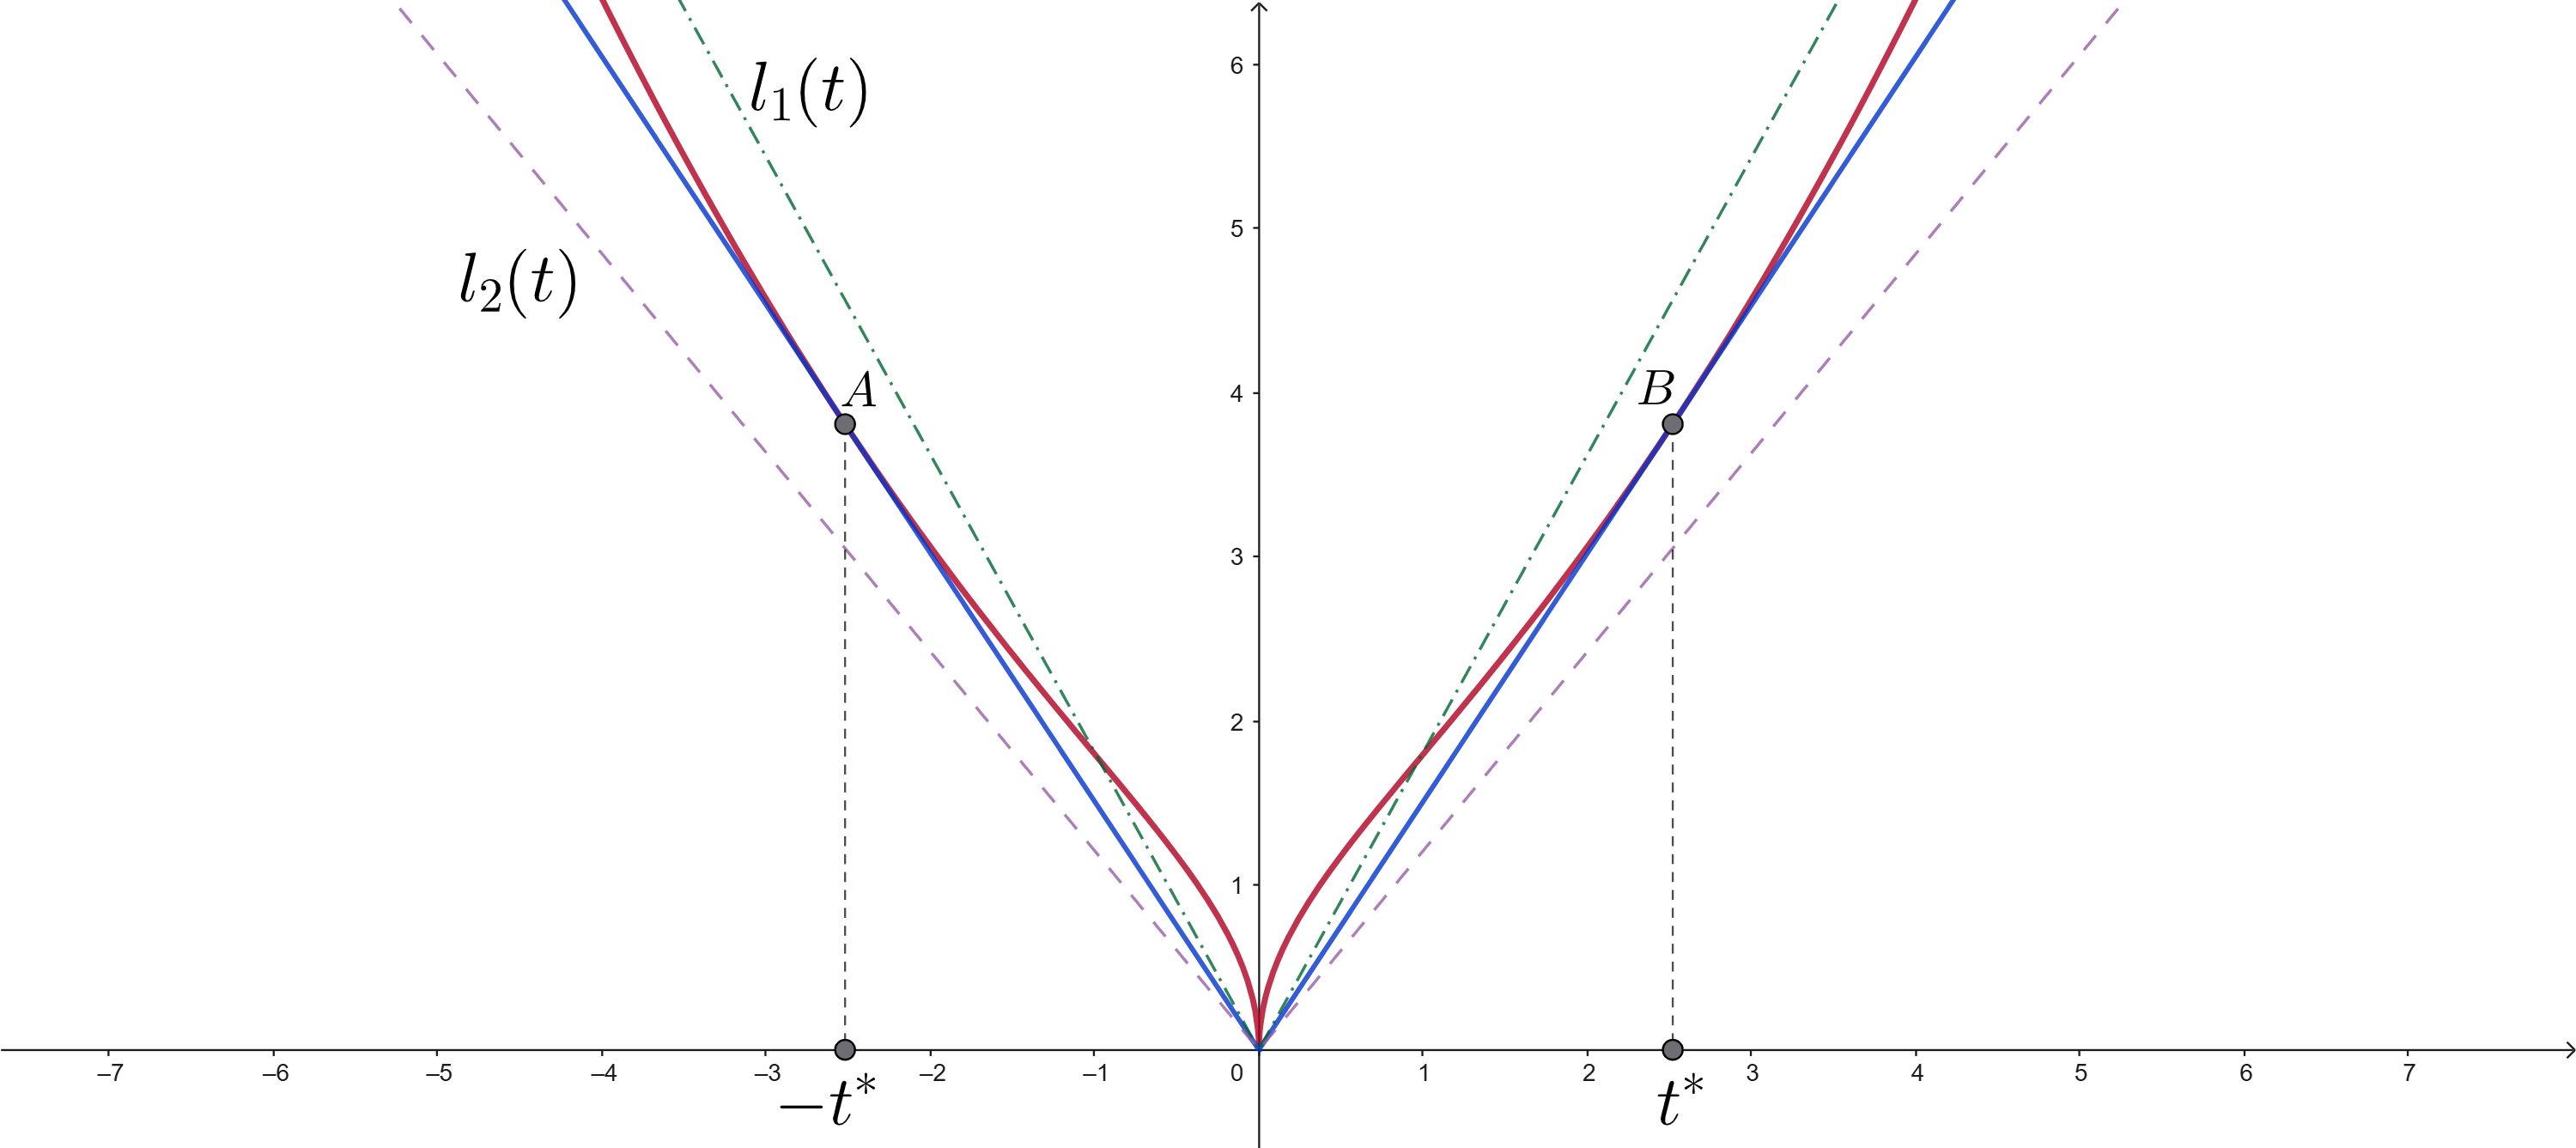
\includegraphics[scale=1]{lqbiconj.png}
     \caption{Graph of the function $\phi_q$ with $q=0.5$, $\alpha=0.4$, $b=1.6$, in red. The two continuous lines in blue represents the greatest continuous affine minorant of $\phi_q$ in $[-t^*, t^*]$. Notice that the points $A$ and $B$ represents the tangency point a which these lines cuts the graph of $\phi_q$. In addition, we see that the two lines $l_1$ and $l_2$ cuts in more that one point the graph of $\phi_q$ (when its slope is greater than $\phi'_q(t^*)$, or is below the blue lines (when its slope is lower than $\phi'(t^*)$.}
     \label{fig:lqbiconj}
 \end{figure}

 \begin{figure}[ht]
     \centering
     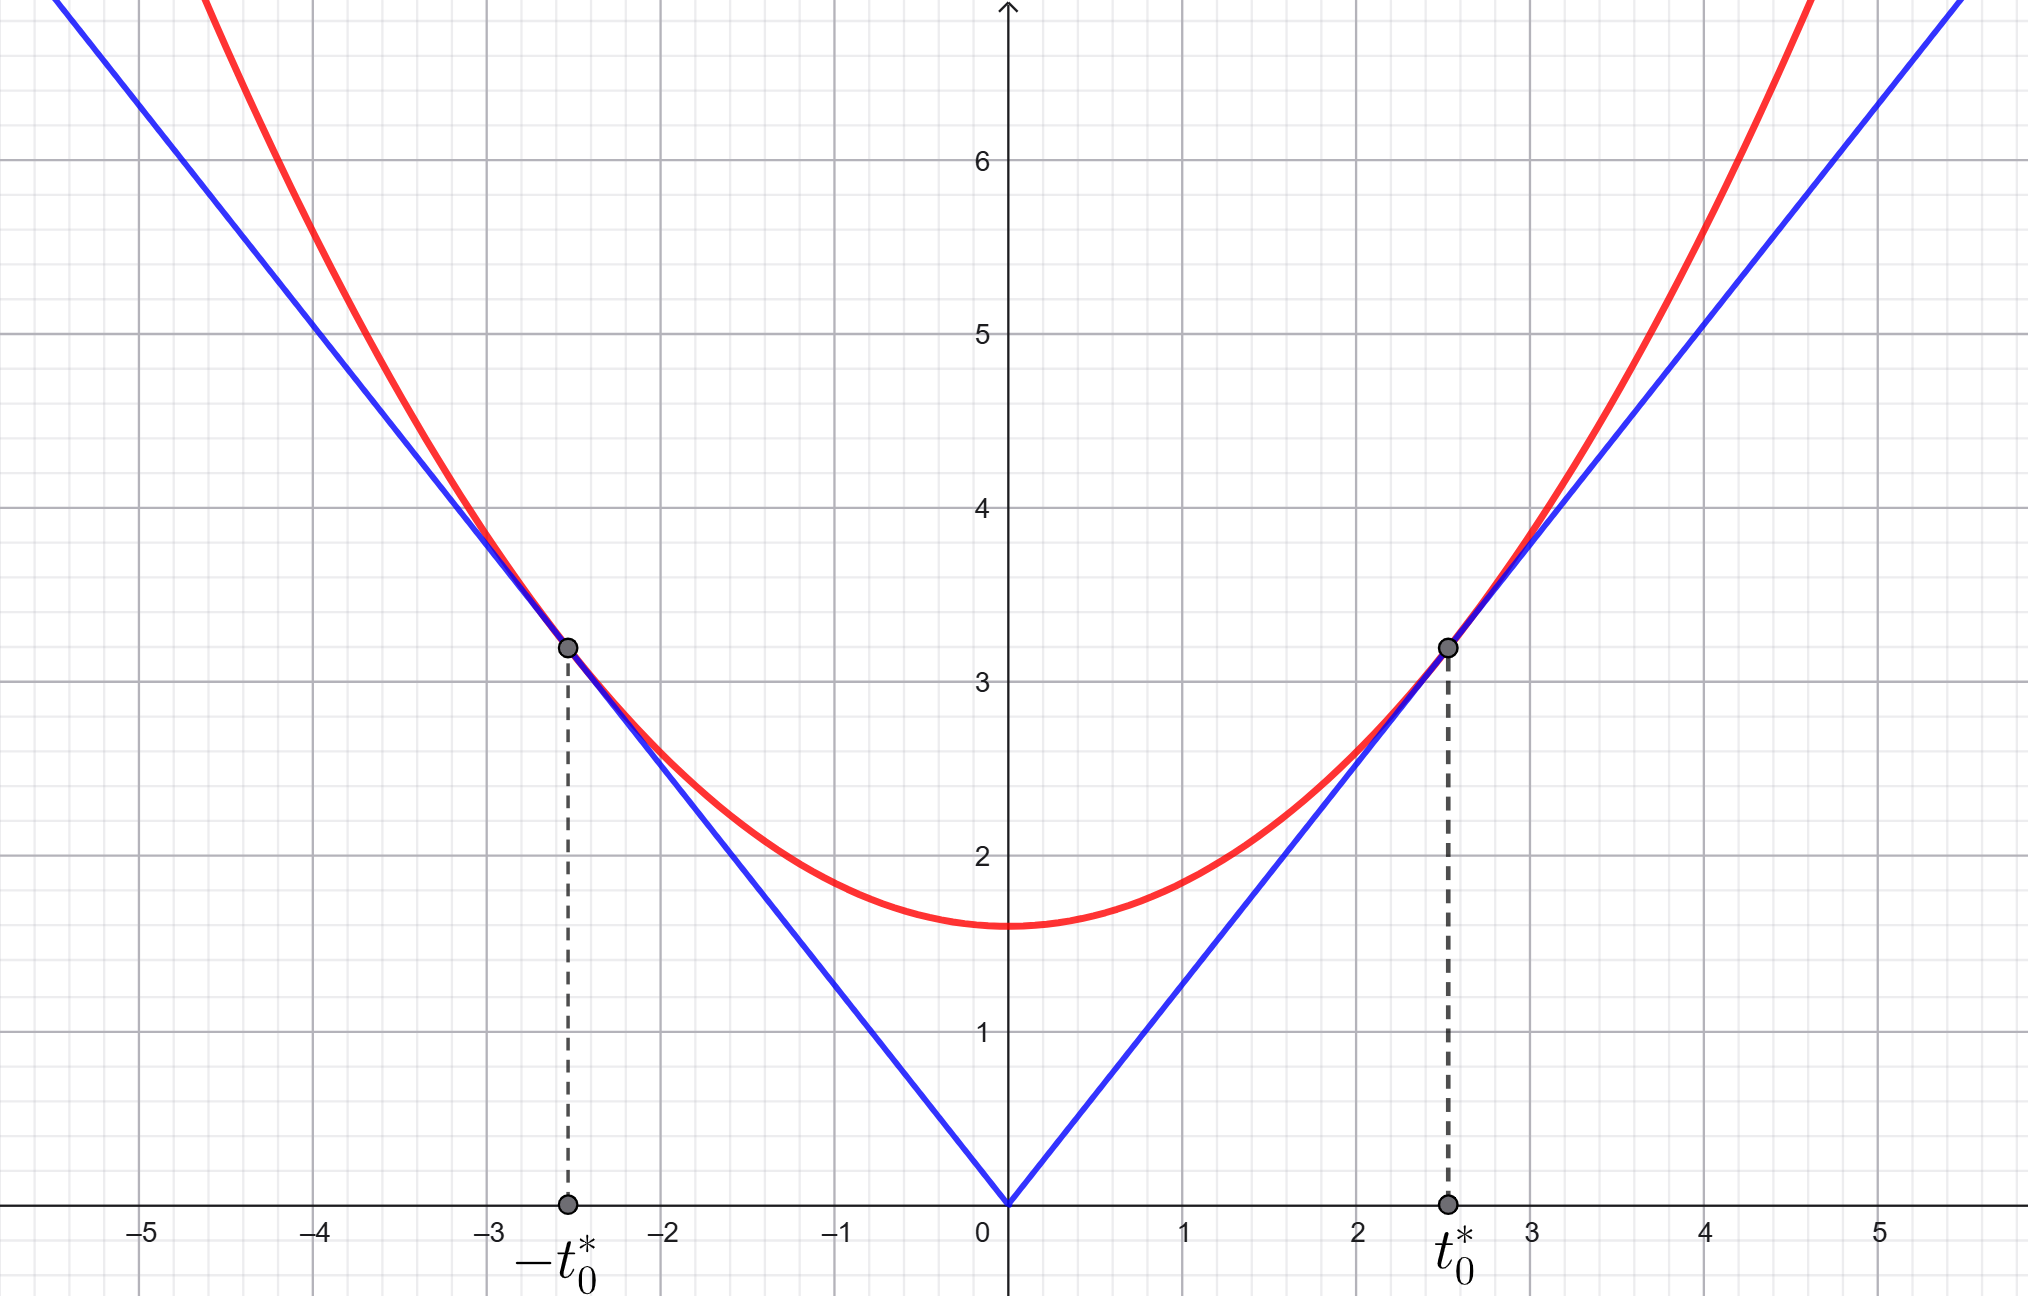
\includegraphics[scale=0.16]{l0biconj.png}
     \caption{Graph of the function $\phi_0$ with $\alpha=0.5$, $b=1.6$, in red. The blue continuous line represents again the greatest affine minorant for $\phi_0$ at $[-t_0^*, t_0^*]$. The construction of the biconjugate for $\phi_0$ is very similar to the case of the biconjugate of $\phi_q$.}
     \label{fig:l0biconj}
 \end{figure}







\section{Numerical algorithms}

In this final section, we present the three numerical algorithms employed to solve the nonconvex optimal control problems investigated in this work. We describe their general structure and report the corresponding convergence results. These methods have proven to be well suited to our framework and have played a key role in validating several theoretical results that were anticipated.

\subsection{The Sequential Quadratic Hamiltonian (SQH) algorithm}

This method is based on the characterization of optimal controls within the framework of the Pontryagin Maximum Principle. Its core idea consists in the iterative solution of a quadratic penalized Hamiltonian constructed from the original optimal control problem. This feature is of particular interest in our setting, since, regardless of the level of penalization imposed on the control, each iteration ultimately reduces to the solution of an optimization problem associated with a quadratic Hamiltonian, that, at least for our studied problems, is equivalent to the solution of unidimensional optimization problems.

Moreover, according to our numerical experiments, this algorithm consistently exhibits the highest robustness and efficiency among the methods considered. Nevertheless, the relatively large number of internal parameters involved introduces a nontrivial tuning challenge. Our experiments reveal that arbitrary or poorly chosen parameter values may lead to unsatisfactory performance, making their careful selection crucial for achieving reliable and accurate results.

The SQH method is not only related to infinite dimensional optimal control problems. In fact, it can be used for solving problems related to ODE's control, differential Nash games, deep learning, stochastics models, and other ones, see \cite{borzi2023}. Even in the theory of optimal control problems governed by PDE's, this method can be used for a large class of these ones, like sparse control problems, state pointwie penalized problems, bilinear problems and more problems. Here, we recall the general framework of the SQH method for control problems governed by elliptic PDE's, and we summarize the results about convergence of the method.

Let $h, g:\mathbb{R}\to [0,\infty)$, $f:\mathbb{R}^3 \to \mathbb{R}$ measurable functions. Consider the problem:

\begin{subequations}\label{eq:sqh_framework_problem}
\begin{equation}
\left\{
\begin{aligned}
\min_{(y,u)\in H_0^1(\Omega)\times L^2(\Omega)} \quad 
& J(y,u) := \int_{\Omega}\big(h(y(x)) + g(u(x))\big)\,dx \\[0.5ex]
\text{s.t.}\quad 
& a(y,v) = \int_{\Omega} f\big(x,y(x),u(x)\big)\,v(x)\,dx,
\quad \forall v \in H_0^1(\Omega), \label{eq:variational_formulation_sqh}\\
& u \in U_{\mathrm{ad}}.
\end{aligned}
\right.
\end{equation}
\end{subequations}




where $a$ is the bilinear operator define in \eqref{eq:bilinear_form}, and $U_{ad}\subset L^2(\om)$. For this kind of problems, we recall the definition of an adjonint state for \eqref{eq:sqh_framework_problem}.A function $p$ is called an adjoint state for \eqref{eq:sqh_framework_problem} if satisfies the equation:
\begin{equation}\label{eq:adjoint_state_sqh}
    a^*(p,z)=\int_{\om}[\partial_y h(y(x))+\partial_y f(x,y(x),u(x))]z(x)\; dx,
\end{equation}
for all $z\in H_0^1(\om)$. Here, $a^{*}$ is the bilinear operator associated to $A^*$ in \eqref{eq:operator_A}.

Since $g,h$ has no more assumptions on their structure, it is possible that \eqref{eq:sqh_framework_problem} have no any solution. However, if we assume that there exist a solution to it, the SQH method demands the following assumptions to guarantee its convergence.
\begin{assumption}\label{assumption:sqh}
    In any compact subset included in the respective domains of definition of
$f$, $h$, and $g$, the following assumptions hold:
\begin{enumerate}
\item
The functions $f$, $\partial_y f$, and $\partial_y h$ are measurable in $x$
and Lipschitz continuous in $y$ and $u$. More precisely, there exist constants
$c_1,c_2,c_3>0$ such that the following inequalities hold uniformly in $x$:
\begin{align*}
|f(x,y_1,u_1)-f(x,y_2,u_2)|
&\le c_1\big(|y_1-y_2|+|u_1-u_2|\big),\\
|\partial_y f(x,y_1,u_1)-\partial_y f(x,y_2,u_2)|
&\le c_2\big(|y_1-y_2|+|u_1-u_2|\big),\\
|\partial_y h(y_1)-\partial_y h(y_2)|
&\le c_3 |y_1-y_2|.
\end{align*}

\item
The solution operators related to the variational formulation  \eqref{eq:variational_formulation_sqh} satisfy the estimates
\[
\|\delta y\|_{L^2(\Omega)} \le c_4 \|\delta u\|_{L^2(\Omega)}, 
\qquad
\|\delta p\|_{L^2(\Omega)} \le c_5 \|\delta u\|_{L^2(\Omega)}.
\]

\item
The adjoint state $p$ which solves the adjoint equation \eqref{eq:adjoint_state_sqh} for given $y$ and $u\in U_{\mathrm{ad}}$
satisfies the uniform bound
\[
\|p\|_{L^\infty(\Omega)} \le c_6.
\]
\end{enumerate}
\end{assumption}
We define the hamiltonian associated to \eqref{eq:sqh_framework_problem} as
\begin{equation}\label{eq:hamiltonian_sqh}
    \mathcal{H}(x,y,u,p):=pf(x,y,u)+h(y)+g(u),
\end{equation}
while the augmented hamiltonian for the SQH is defined as
\begin{equation}
    \mathcal{H}_{\epsilon}(x,y,u,v,p):=\mathcal{H}(x,y,u,p)+\varepsilon (u-v)^2,
\end{equation}
defined for a fixed $\varepsilon>0$. With this augmented hamiltonian, the SQH method is define in Algorithm  \ref{alg:sqh}.

An important feature for ensuring well-definedness of the SQH algorithm is that in step 5. the minimization problem returns a measurable function for all $k=1,2,\cdots$. This fact is not general true for general functions $g, h $ and $f$. However, in our context, we will prove later that our election of $g, h$ produces a sequence of measurable functions $u^k$, given a measurable initial election $u^0$. 

\begin{algorithm}
\caption{Sequential Quadratic Hamiltonian (SQH) method for elliptic optimal control problems}
\label{alg:sqh}
\begin{algorithmic}[1]
\Require Initial control $u^0$, maximal number of iterations $k_{\max}$, tolerance $\kappa>0$, parameters $\tau>0$, $\varepsilon>0$, $\sigma>1$, $\eta>0$, and $\xi\in(0,1)$.
\State Set $k\gets 0$.
\State Compute the state $y^0$ as the solution of 
\[
a(y,v)=\int_{\Omega} f\big(x,y,u^0(x)\big)\,v(x)\,dx,\qquad \forall v\in H_0^1(\om).
\]
\While{$k<k_{\max}$ \textbf{and} $\tau>\kappa$}
    \State Compute $p^k$ as the solution of the adjoint problem:
    \[
    a^*(p,v)=\int_{\Omega}\Big(\partial_y h\big(y^k(x)\big)
    +\partial_y f\big(x,y^k(x),u^k(x)\big)\,p(x)\Big)\,v(x)\,dx,
    \qquad \forall v\in H_0^1(\om).
    \]
    \State For a.e. $x\in\Omega$, determine $u^{k+1}(x)\in U_{\mathrm{ad}}$ such that
    \[
    u^{k+1}(x)\in\arg\min_{w\in U_{\mathrm{ad}}} \mathcal{H}_{\varepsilon}\big(x,y^k(x),w,u^k(x),p^k(x)\big).
    \]
    \State  Compute $y^{k+1}$ as the solution of
    \[
    a(y,v)=\int_{\Omega} f\big(x,y,u^{k+1}(x)\big)\,v(x)\,dx,\qquad \forall v\in H_0^1(\om).
    \]
    \State Compute $\tau \gets \|u^{k+1}-u^k\|_{L^2(\Omega)}^2$.  
    \If{$J\!\left(y^{k+1},u^{k+1}\right) - J\!\left(y^k,u^k\right) > -\eta\,\tau$}
        \State Increase $\varepsilon \gets \sigma\,\varepsilon$ and \textbf{go to} Step 2.
    \ElsIf{$J\!\left(y^{k+1},u^{k+1}\right) - J\!\left(y^k,u^k\right) < -\eta\,\tau$}
        \State Decrease $\varepsilon \gets \xi\,\varepsilon$.
    \EndIf
    \State Update $k\gets k+1$.
\EndWhile
\end{algorithmic}
\end{algorithm}
The next result establish a minimising property for the SQH algorithm. This result can be found in \cite[Theorem 7.3]{borzi2023}

\begin{theorem}\label{thm:sqh_minimizing}
Let $(y^k,u^k)$ and $(y^{k+1},u^{k+1})$ be generated by the SQH method,
Algorithm~\ref{alg:sqh}, and let $u^{k+1}$ and $u^k$ be measurable.
Assume that Assumption~\ref{assumption:sqh} hold.
Then, there exists $\theta>0$, independent of $\varepsilon$, $k$, and $u^k$,
such that for the parameter $\varepsilon>0$ currently chosen by
Algorithm~\ref{alg:sqh}, the following estimate holds:
\begin{equation}\label{eq:sqh_descent}
J\big(y^{k+1},u^{k+1}\big) - J\big(y^k,u^k\big)
\le -(\varepsilon-\theta)\,\|u^{k+1}-u^k\|_{L^2(\Omega)}^2 .
\end{equation}
In particular, it holds that
\[
J\big(y^{k+1},u^{k+1}\big) - J\big(y^k,u^k\big)
\le -\eta\,\tau
\quad \text{for } \varepsilon \ge \theta+\eta,
\]
where
\[
\tau := \|u^{k+1}-u^k\|_{L^2(\Omega)}^2 .
\]
\end{theorem}

Finally, we provide the result of convergence for this Algorithm. The proof of this one can be found in \cite[Theorem 7.4]{borzi2023}
\begin{theorem}\label{thm:sqh_convergence}
Let the assumptions of Theorem~\ref{thm:sqh_minimizing} be fulfilled.
Assume that in Algorithm~\ref{alg:sqh}, at every $k$-th iterate,
the parameter $\varepsilon=\theta+\eta$ is chosen.
Then, the following statements hold:
\begin{enumerate}[label=\textup{(\alph*)}]
\item
The sequence $\big(J(y^k,u^k)\big)_{k=0,1,2,\dots}$ is monotonically decreasing
and converges to some value
\[
\hat J \ge \inf_{u\in U_{\mathrm{ad}}} \hat J(u).
\]

\item
It holds that
\[
\lim_{k\to\infty} \|u^{k+1}-u^k\|_{L^2(\Omega)} = 0.
\]
\end{enumerate}
\end{theorem}

\subsection{The Difference of Convex functions (DC) algorithm}

The theory of Difference of Convex  (DC) functions was developed in the later 70's by Toland first, and Singer \cite{toland, singer}, in the context of convex maximization theory in finite dimensional spaces. Later, several deep results and algorithms based on this theory was proposed by Pham Dinh Tao and Le Thi Hoai An in \cite{tao}. Inspired by this work, the infinite dimensional case for finding existence of solutions, necessary and sufficient optimal conditions of DC problems in the context of indefinite quadratic problems are deveolped in \cite{bonnans, yen}. The later novelty paper \cite{lim} deals with DC algorithms in general Hilbert spaces, proving sufficient conditions for the convergence of this algorithm and given a rate of convergence for indefinite quadratic programs. 

One of the most appealing features of DC algorithms lies in the formulation and solution of two primal–dual problems, for which a wide range of numerical methods have been extensively studied and optimized. In the context of nonconvex optimal control problems, several works have addressed this approach; see, for instance, \cite{hinze, ioffe}. For optimal control problems involving $L^q$-type penalizations, the work \cite{merino2019} is particularly relevant. There, a Huber-type regularization is introduced to incorporate the nonconvex penalty, and by expressing the cost functional as the difference of two convex functions, a DC scheme based on two primal–dual problems is developed. One of these subproblems involves an $L^1$-penalized optimal control problem, for which a variety of efficient numerical solution methods are available.
We consider the general setting of the DC algorithm. For a general Hilbert space $X$, let $g, h: X\to \mathbb{R}$ two convex and lower semicontinuous functions. Consider the minimization problem
\begin{equation}\label{eq:dc_formulation}
    \inf_{x\in X} f(x):=g(x)-h(x).
\end{equation}
\eqref{eq:dc_formulation} is called a DC program. Associated with this problem, we formulate the dual problem associated to it as
\begin{equation}\label{eq:dc_dual_formulation}
    \inf_{x\in X} \widetilde{f}(x):=h^{*}(x)-g^{*}(x).
\end{equation}
It can be shown that \eqref{eq:dc_formulation} and \eqref{eq:dc_dual_formulation} has the same optimal value, see \cite[Proposition 2.5]{lim}. Moreover, the following first order optimally condition, whcih is important for developing the DC algorithm, follows.
\begin{proposition}\label{prop:first_order_condition_dc}
    If $x^*$ is a local solution for \eqref{eq:dc_formulation}, then $\partial h(x^*)\subset \partial g(x^*)$.
\end{proposition}

The following algorithm is called the DC algorithm. 

\begin{algorithm}[ht]
\caption{DC Algorithm (DCA) in Hilbert spaces}
\label{alg:dca}
\begin{algorithmic}[1]
\Require DC decomposition $F = g - h$, where $g,h : X \to \mathbb{R}\cup\{+\infty\}$ are proper, lower semicontinuous, convex functions.
\Require Initial point $x^0 \in \operatorname{dom} g$.
\State Set $k \gets 0$.
\While{stopping criterion not satisfied}
    \State
    Choose $y^k \in \partial h(x^k)$, provided that $\partial h(x^k)\neq \emptyset$.
    \State 
    Choose $x^{k+1} \in \partial g^*(y^k)$, provided that $\partial g^*(y^k)\neq \emptyset$.
    \State Update $k \gets k+1$.
\EndWhile
\end{algorithmic}
\end{algorithm}
Before to establish the properties of the DC algorithm, we introduce the concept of modulus of convexity. 
\begin{definition}\label{def:modulus_convexity}
    Lef $f:X\to \mathbb{R}$ a convex function. Its modulus of convexity is defined as
    \[
    \rho(f)=\sup \l\{\rho\ge 0: f(\cdot)-\frac{\rho}{2}\norm{\cdot}^2 \mbox{ is a convex function over }X \r\}
    \]
\end{definition}

Consider the pair of problems \eqref{eq:dc_formulation} and \eqref{eq:dc_dual_formulation}. If $\rho(g) > 0$ 
(resp., $\rho(g^*) > 0$), let $\rho_1$ (resp., $\rho_1^*$) be a real number such that
\[
0 \le \rho_1 < \rho(g) \quad (\text{resp., } 0 \le \rho_1^* < \rho(g^*)).
\]
If $\rho(g) = 0$ (resp., $\rho(g^*) = 0$), let $\rho_1 = 0$ (resp., $\rho_1^* = 0$).
If $\rho(h) > 0$ (resp., $\rho(h^*) > 0$), let $\rho_2$ (resp., $\rho_2^*$) be a real number such that
\[
0 \le \rho_2 < \rho(h) \quad (\text{resp., } 0 \le \rho_2^* < \rho(h^*)).
\]
If $\rho(h) = 0$ (resp., $\rho(h^*) = 0$), let $\rho_2 = 0$ (resp., $\rho_2^* = 0$). Finally, define
\[
d x^k := x^{k+1} - x^k, \qquad d y^k := y^{k+1} - y^k,
\]
and denote the optimal value of \eqref{eq:dc_formulation} by $\alpha$, that is,
\[
\alpha := \inf \{ f(x) = g(x) - h(x) : x \in H \}.
\]
The following Theorem establishes the convergence properties of the DC algorithm. Its proof can be found in \cite[Theorem 2.11]{lim}.
\begin{theorem}\label{thm:convergence_dc}
Assume that the iteration sequences $(x^k)$ and $(y^k)$ are generated by the DCA. We have
\begin{enumerate}
\item[(i)]
\begin{align*}
(g - h)(x^{k+1})
&\le (h^* - g^*)(y^k)
- \max \left\{ \frac{\rho_2}{2} \|d x^k\|^2, \frac{\rho_2^*}{2} \|d y^k\|^2 \right\} \\
&\le (g - h)(x^k)
- \max \Bigg\{
\frac{\rho_1 + \rho_2}{2} \|d x^k\|^2,\,
\frac{\rho_1^*}{2} \|d y^{k-1}\|^2 \\
&\hspace{3cm}
+ \frac{\rho_2}{2} \|d x^k\|^2
+ \frac{\rho_1^*}{2} \|d y^{k-1}\|^2
+ \frac{\rho_2^*}{2} \|d y^k\|^2
\Bigg\}.
\end{align*}

\item[(ii)]
\begin{align*}
(h^* - g^*)(y^{k+1})
&\le (g - h)(x^{k+1})
- \max \left\{ \frac{\rho_1}{2} \|d x^{k+1}\|^2, \frac{\rho_1^*}{2} \|d y^k\|^2 \right\} \\
&\le (h^* - g^*)(y^k)
- \max \Bigg\{
\frac{\rho_1^* + \rho_2^*}{2} \|d y^k\|^2,\,
\frac{\rho_1}{2} \|d x^{k+1}\|^2 \\
&\hspace{3cm}
+ \frac{\rho_2}{2} \|d x^k\|^2
+ \frac{\rho_1^*}{2} \|d y^k\|^2
+ \frac{\rho_2}{2} \|d x^k\|^2
\Bigg\}.
\end{align*}

\item[(iii)]
If $\alpha$ is finite, then $\{(g-h)(x^k)\}$ and $\{(h^*-g^*)(y^k)\}$ are decreasing sequences that converge to the same limit $\beta \ge \alpha$.

\item[(iv)]
Assume that $\alpha$ is finite and that $(x^k)$ and $(y^k)$ are bounded.  
If $\{x^k\}$ contains a strong limit point $x^*$ (resp., $(y^k)$ contains a strong limit point $y^*$), then there is a weak limit point $y^*$ of $\{y^k\}$ (resp., $x^*$ of $\{x^k\}$) such that
\[
(x^*, y^*) \in [\partial g^*(y^*) \cap \partial h^*(y^*)]
\times
[\partial g(x^*) \cap \partial h(x^*)].
\]

Moreover, if $\rho_1 + \rho_2 > 0$ (resp., $\rho_1^* + \rho_2^* > 0$), then
\[
(g - h)(x^*) = (h^* - g^*)(y^*) = \beta.
\]
\end{enumerate}
\end{theorem}





\subsection{The Semismooth Newton (SSN) algorithm}

The semismooth Newton (SSN) method is formulated within the framework of solving optimization problems 
of the form

\begin{equation}
\min_{y,u\in U\times Y} J(y,u)
\quad \text{subject to } E(y,u)=0 \text{ and } g(y,u) \in C.
\end{equation}


where $U$ and $Y$ denote the control and state spaces, respectively. Here, $J$ represents a cost functional, 
$E$ denotes a partial differential equation linking the control $u$ and the state $y$, and $g(y,u)\in C$ 
represents a generic inequality-type constraint. The mapping $g$ takes values in a vector of $m$ measurable 
real-valued functions, while $C\subset \mathbb{R}^{m}$ is a closed and convex set.
The goal of the method is to reformulate the stated problem, starting from first-order necessary optimality 
conditions, into an equivalent system of equations of the form $F(u)=0$, where $F$ must be a semismooth 
function—a concept that will be detailed later.

As pointed out in \cite{ulbrich}, the method was originally designed to address problems of this type in 
finite-dimensional spaces. Some early contributions in this direction can be found in \cite{mifflin, qi, pang}, 
with \cite{mifflin} being the first work to introduce the concept of semismoothness in finite-dimensional 
settings. Extensions of several concepts from the theory of semismooth operators to Banach spaces were later 
developed in works such as \cite{kummer, robinson, chen}. However, in \cite{ulbrich}, the use of superposition 
operators makes it possible to transfer many essential features of semismooth Newton methods from 
finite-dimensional spaces to general Banach spaces.

The SSN method has been widely applied to optimal control problems governed by linear elliptic partial 
differential equations and penalized with an $L^1$ term. In \cite{stadler}, it is shown that, under a 
reformulation of the problem via a semismooth function, the method converges superlinearly, provided that 
the initial iterate is sufficiently close to the solution. The convexity of the problem and the coercivity 
of the differential operator play a fundamental role in establishing the convergence of the method. 
In \cite{merino2021}, a direct application of the method is presented for problems involving $L^q$
 penalization, with $q\in (0,1)$. A Huber-type regularization is introduced in order to show that the 
 problem can be reformulated through a semismooth Newton function. However, no convergence proof of the 
 method is provided therein.

A generalization of Stadler’s analysis to problems governed by semilinear partial differential equations 
is studied in \cite{casasmateos}. Nevertheless, the convergence proof in this setting requires the 
development of second-order optimality conditions. For linear problems with $L^q$ penalization, one may 
follow a combination of methods based on the results presented in \cite{stadler} and \cite{casasmateos}. 
Hoever, a possible estension to the semilinear case is particularly difficult, since there exists only
second order conditions like the presented in \cite{casas-wachsmuth}, which not implies directly enough 
conditions to establish the convergence of the method.

Before the introduction of the SSN algorithm, we present the definition of a semismooth function.

\begin{definition}\label{def:semismooth}
Let $X$ and $Y$ be Banach spaces, and let $V \subset X$ be an open set.
Let $f : V \to Y$ and
\[
\partial^* f : V \rightrightarrows \mathcal{L}(X,Y)
\]
be a set-valued mapping such that $\partial^* f(y) \neq \emptyset$ for all $y \in V$.
We say that $f$ is $\partial^*$-semismooth at $y \in V$ if $f$ is continuous at $y$ and
\[
\sup_{M \in \partial^* f(y+s)}
\| f(y+s) - f(y) - Ms \|_{Y}
= o(\|s\|_{X})
\quad \text{as } \|s\|_{X} \to 0.
\]
Moreover, we say that $f$ is $\alpha$-order $\partial^*$-semismooth at $y$, $0 < \alpha \le 1$,
if $f$ is continuous near $y$ and
\[
\sup_{M \in \partial^* f(y+s)}
\| f(y+s) - f(y) - Ms \|_{Y}
= O(\|s\|_{Y}^{1+\alpha})
\quad \text{as } \|s\|_{X} \to 0.
\]
\end{definition}

Now, assume that $f:V\subset X\to Y$ is a $\partial^*$-semismooth function. 
We are interested in solving the equations
\begin{equation}\label{eq:ssn_equation}
f(y)=0.
\end{equation}
The following algorithm, called SSN algorithm, is implemented in order to find the root of $f$ as 
shown in the last equation stablish. We assume that $Y$ is continuously
and densely embedded in a bigger space $Y_0$.

\begin{algorithm}[ht]
\caption{Semismooth Newton method}
\label{alg:ssn_ulbrich}
\begin{algorithmic}[1]
\State Choose an initial point $y_0 \in V$ and set $k = 0$.
\While{stopping criterion not satisfied}
\State Choose $M_k \in \partial^* f(y_k)$ and compute $s_k \in Y_0$ from
\[
M_k s_k = - f(y_k).
\]
\State Set $y_{k+1}^{0} = y_k + s_k$.
\State Perform a smoothing step: $Y_0 \ni y_{k+1}^{0} \mapsto y_{k+1} = S_k\!\left(y_{k+1}^{0}\right) \in Y$.
\If{$y_{k+1} = y_k$}
\State \textbf{stop} with result $y^* = y_{k+1}$.
\EndIf
\State $k \gets k+1$.
\EndWhile
\end{algorithmic}
\end{algorithm}

The following assumption is crucial for the convergence of the SSN algorithm.
\begin{assumption}\label{ass:ulbrich_3_12}
The space $Y$ is continuously and densely embedded in a Banach space $Y_0$ such that:
\begin{enumerate}
\item[(a)] \emph{(Regularity condition)}  
The operators $M_k$ map $Y_0$ continuously into $Z$ with bounded inverses, and there exists a constant
$C_{M^{-1}} > 0$ such that
\[
\|M_k^{-1}\|_{\mathcal{L}(Z,Y_0)} \le C_{M^{-1}}.
\]

\item[(b)] \emph{(Smoothing condition)}  
The smoothing steps in step 5 satisfy
\[
\|S_k(y_{k+1}^0) - \bar y\|_Y \le C_S \|y_{k+1}^0 - \bar y\|_{Y_0}
\]
for all $k$, where $\bar y \in Y$ solves~(3.7).
\end{enumerate}
\end{assumption}

Under this Assumption, the following Theorem follows. For a proof 
of this result, see \cite[Theorem 3.13]{ulbrich}

\begin{theorem}\label{thm:ssn_convergence}
Let $f : Y \supset V \to Z$ be an operator between Banach spaces defined on the open set $V$,
with generalized differential $\partial^* f : V \rightrightarrows \mathcal{L}(Y,Z)$.
Denote by $\bar y \in V$ a solution of \eqref{eq:ssn_equation} and let Assumption~\ref{ass:ulbrich_3_12} hold.
Then the following assertions are valid:
\begin{enumerate}
\item[(a)]
If $f$ is $\partial^*$-semismooth at $\bar y$, then there exists $\delta > 0$ such that,
for all $y_0 \in \bar y + \delta B_Y$,
Algorithm \ref{alg:ssn_ulbrich} either terminates with $y^* = y_k = \bar y$ or generates a sequence
$(y_k) \subset V$ that converges $q$-superlinearly to $\bar y$ in $Y$.

\item[(b)]
If in~(a) the mapping $f$ is $\alpha$-order $\partial^*$-semismooth at $\bar y$,
$0 < \alpha \le 1$, then the $q$-order of convergence is at least $1+\alpha$.
\end{enumerate}
\end{theorem}
